\section{Image Data Analysis}
\subsection{Introduction}
\noindent
After exploring behavior data, we proceed to image data analysis.  First we need to apply convolution to connect behavior stimuli and neural activity. Then we can run general linear regression to find activated voxels across time course. Using hypothesis testing, we can actually locate and visualize the activated voxels. After finishing basic steps, we try to apply noise modeling and PCA to compare the MRSS so that we can finally decide our design matrix.

\subsection{Methods}
Here are some of the methods (this needs to be updated soon as well.)

\subsubsection {Convolution}
Our experiment is event-oriented. The subject is shown with the different conditions such as gain and loss amounts over random time. After being provided with the conditions, the blood flow responses starts to fluctuate. To predict the fMRI signal to an event, we need to predict the hemodynamic responses to neural activity. A predictor neural time course is typically obtained by convolution of a condition of the experiment with a standard hemodynamic response function. With this predictor, we build our design matrix for our general linear model on each voxel of a subject's brain. To produce such predictor, we practiced two different approaches.
\begin{itemize}
\item  Convolving with canonical HRF \\
A typical BOLD response to a single, impulsive stimulation resembles a linear combination of two Gamma function. This would model a signal is instantly at its peak level at the onset of a given condition and instantly undershoot back to around baseline with the offset of a condition. We can use this hemodynamic response function as a canonical one. Generally, the canonical HRF should be a good fit if we believe the subjects to be normal in many cortical regions. Using this canonical HRF will help us to find how much the canonical HRF has to be scaled enough to account for the signal. However, we want to be more in detail as long as the onsets of the HRF can happen in the middle of volumes due to the conditions given at different times. The amplitudes vary according to the parametric gain and loss conditions. Thus, the true shape of HRF for each subject should vary.


\item  Convolving at finer time resolution \\
Therefore, we would make a neural and hemodynamic regressor at a finer time resolution than the TRs, and later sample this regressor at the TR onset times. This refers that stimulus onsets do not have to be synchronized with scan TRs.
\end {itemize}


\subsubsection {GLM}
The first matrix we get from convolution has five columns, which correspond to a column of ones and 4 cond.txt files in our dataset, respectively. After we get the convolution matrix, we use it as our design matrix to run the generalized linear regression on the image data. The dimension of our data is (64, 64, 34, 240), so, first we reshape our data into 2 dimensional array, which has the shape of (64*64*34, 240); the first dimension corresponds to 3-dimensional voxel indices and the second dimension corresponds to the time slice. Then we pass our design matrix into the glm function to calculate the related beta hats. Thus, there are in total 139624 beta hats that we get from the regression correspond to the first three dimensions of our image data. For example, the first beta hat contains the information about the voxel (0,0,0). Then we turn the beta hats back into 4-dimensional shape and run the diagnostic functions on the 4-d beta hats. Based on the predictors, we can calculate the fitted values and then the residuals. We use the MRSS of the first three dimensions as a measurement of our regression; in general, a smaller MRSS indicates a better performance of the regression model. 

\subsubsection {Smoothing}
After we tried with the normal convolution matrix, we also generated high resolution convolution matrix and used it for linear regression. It turned out that the MRSS is just reduced by a little bit. Then we write a smoothing function to implement the multidimensional Gaussian filter on our data. We repeat the same procedures as what we have done in normal convolution on the smoothed data and the MRSS are reduced sharply. Therefore, we concluded that the smoothing method is a good pre-processing when we do the linear regression. 

\subsubsection {Hypothesis Testing}
From linear regression, we can get t-statistics for different conditions(task on/off, gain, loss, distance).For each condition, we will have a 3D t-statistics matrix. For visualization, we first added mask based the mean voxel and the histogram. We set a boolean mask which takes larger than 375. Also we used smooth function and better color txt to generate a better image. Then we plotted the t statistics map for gain/loss. 
\begin{figure}[H]
\begin{subfigure}{.5\textwidth}
  \centering
  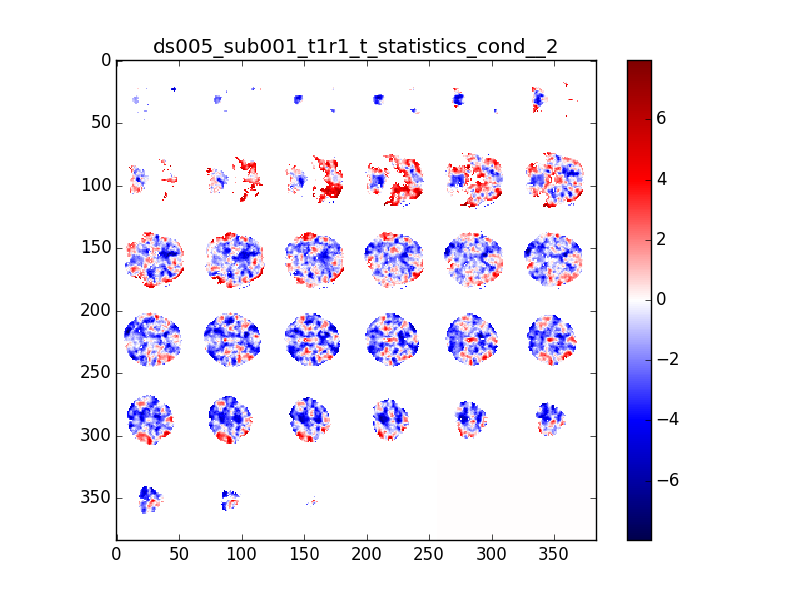
\includegraphics[width=.8\linewidth]{../fig/t_test/ds005_sub001_t1r1_t-test_cond2.png}
  \caption{Gain}
  \label{fig:sfig1}
\end{subfigure}%
\begin{subfigure}{.5\textwidth}
  \centering
  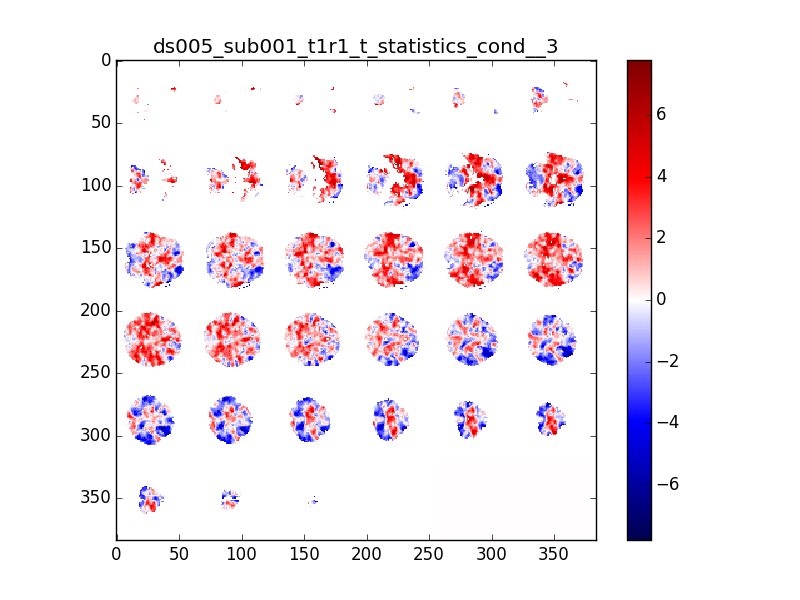
\includegraphics[width=.8\linewidth]{../fig/t_test/ds005_sub001_t1r1_t-test_cond3.png}
  \caption{Loss}
  \label{fig:sfig2}
\end{subfigure}
\caption{t statistics map for gain/loss (subject1)}
\label{fig:fig}
\end{figure}

\begin{figure}[H]
\begin{subfigure}{.5\textwidth}
  \centering
  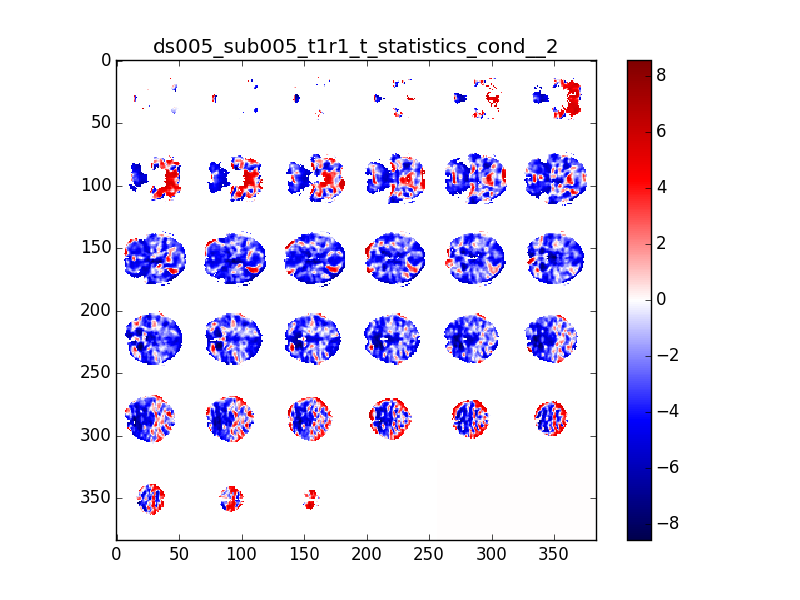
\includegraphics[width=.8\linewidth]{../fig/t_test/ds005_sub005_t1r1_t-test_cond2.png}
  \caption{Gain}
  \label{fig:sfig1}
\end{subfigure}%
\begin{subfigure}{.5\textwidth}
  \centering
  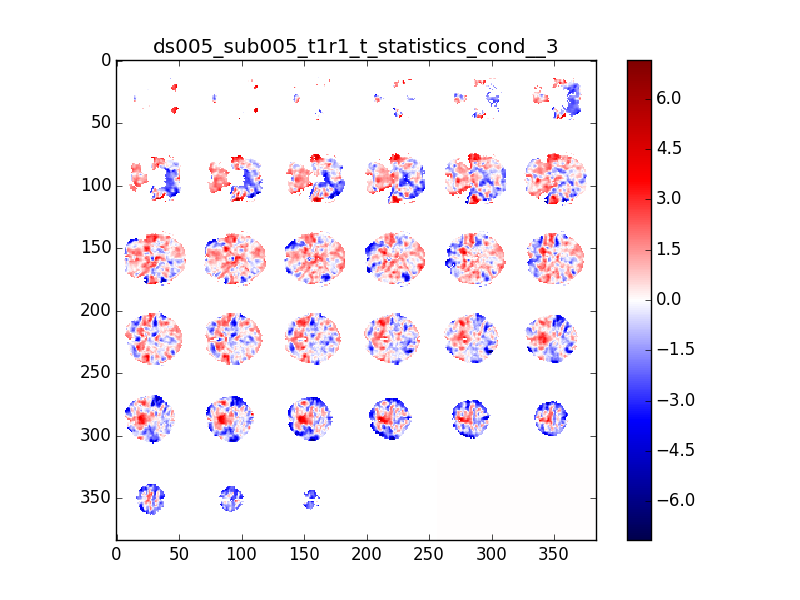
\includegraphics[width=.8\linewidth]{../fig/t_test/ds005_sub005_t1r1_t-test_cond3.png}
  \caption{Loss}
  \label{fig:sfig2}
\end{subfigure}
\caption{t statistics map for gain/loss (subject5)}
\label{fig:fig}
\end{figure}
\noindent
The larger the t-statistics, the more significant. Thus the red spots represents the activated voxels for gain and loss. For subject 1, gain has more activated voxels. However, for subject 5, loss has more activated voxels.

\subsubsection {Noise Model}

\subsubsection {PCA}

\subsection {Results}
In terms of convolution, to analyze the difference between two approaches, we compare the MRSS from two linear regressions on image data of three subjects (1,2,3) using convolution predictors from two different approaches. In the below table, we see the MRSS from linear regression using the latter approach has slightly lower residuals compared to the former method. This makes sense because, using the latter method, we are able to more elaborately preprocess the data.



